%実験は過去形に統一
\chapter{提案手法}

一般に、音楽で特定の音色への変換を行うことは難しいが、次の三つの要素に分解することで単音での音色の変換を音楽へと適用することが可能であると考えられる。また、三つの要素とは、楽器の重ね合わせ・音の重ね合わせ・時間方向の音の繋ぎ方であり、それぞれについて具体的に以下で説明をする。

\begin{description}

\item[楽器の重ね合わせ]\mbox{}

音楽はそれぞれの楽器により奏でられた音の重ね合わせになっている。楽器ごとに音色は異なるので楽器ごとの音波に分解して音色変換を行う~(音源分離)~が必要であると考えられる。なお、楽曲の作成時に楽器ごとに分離したデータ~(パラデータ)~で保存しておけば、音源分離を行わずに直接楽器ごとの音波を利用できる。

\item[音の重ね合わせ]\mbox{}

ある単位時間の音に注目した時、楽器ごとの音波に分解してもその単位時間で異なった高さや大きさの音の重ね合わせになっていることがある。この場合は、今回の提案手法で用意したデータセット以外に和音のデータセットも加えて学習させることで表現可能であると考えられる。

\item[時間方向の音の繋ぎ方]\mbox{}

%他の工夫があるかも

楽器ごとの音波に分解し単位時間の音が表現できた時、時間方向に音を繋ぐ必要がある。時間方向については先程定めた単位時間で区切って順に変換していくことで可能であると 考えている。また、区切るのみでの変換が難しい場合は自己回帰モデルを取り入れるなどの工夫が必要であると考えている。

\end{description}


\section{データセット}

本節では、データセットの作成方法及びその形式についての説明を行う。

\subsection{データセットの作成方法}

楽譜作成ソフトのMuseScore\footnote{\url{https://musescore.org/}}により、A0からC8までの半音を88音生成した。この88音は最も一般的な音域として今回の実験では選んだ。また、ギターからハープの音へと音色の変換を行ったので、そのどちらも88音を生成した。

\subsection{データ形式}

音のファイル形式としては非圧縮形式のWAV形式を用いる。WAV形式は音波の波形データを直接保持しているために扱いやすいので本論文では採用した。また、WAV形式は音波の波形データ以外にメタデータも持つ。以下では、本論文で関係のあるメタデータについて説明する。

\begin{description}

\item[サンプリング周波数]\mbox{}

サンプリング周波数とは、デジタル信号の1秒あたりの標本化の回数のことである。本論文では44100Hzに固定して実験を行う。

\item[サンプリング数]\mbox{}

サンプリング数とは、デジタル信号の標本化の合計の回数のことである。本論文では44100回に固定して実験を行う。

\item[量子化ビット数]\mbox{}

量子化ビット数とは、デジタル信号の細かさを表現するビット数のことである。本論文では16bitに固定して実験を行う。

\item[チャンネル数]\mbox{}

チャンネル数とは、モノラルな音声の出力の総数のことである。本論文では1に固定して実験を行う。

\end{description}

\section{手法}

Pix2pixを用いて十分に音色が異なると考えられるギターからハープへの音の変換を行った。学習と評価の際のパラメータは付録\ref{sec:appendix}の\ref{sec:appendix_params}節に示す。また、本研究で行うニューラルネットワークの学習にはAdamを用いた。

%\subsection{ニューラルネットワークのモデル}

%本実験では、Pix2pixを元にしたニューラルネットワークのモデルを作成した。


%全体,generator,discriminatorの順に書く
%できれば図があると良い

%normalize()とdenormalize()をしていることも書く

\subsection{生成モデルの表現力の評価}

生成モデルの表現力を測るために学習データと評価データに同じ88音のデータセットを用いて実験を行う。また、88音と小さいサイズのデータセットへの過学習を防ぐためにそれぞれのデータの振幅を乱数で変化させる工夫をした。

具体的には、乱数のシードをあらかじめ固定した後、各エポックで学習データとして与えるデータごとに振幅を$c$倍した。$c$の範囲は$[0.3,1]$であり、一様乱数により$c$を生成している。

\subsection{生成モデルの汎化能力の評価}

一般に、単音の音色変換において任意の高さと大きさの音を学習データとして用意するのは不可能である。従って、未知のデータも適切に処理できるニューラルネットワークを構築する必要がある。本手法のニューラルネットワークが未知のデータも適切に処理できるか調べるため、88音のうち3/4を学習データ,1/4を評価データとする4分割交差検定を行う。この際のデータセットの分割方法は付録\ref{sec:appendix}の\ref{sec:appendix_split}節に示した。また、先程の実験と同様、各エポックで学習データとして与えるデータごとに振幅を$c \in [0.3,1]$倍して学習を行った。

\section{実験結果}

本節では、実験結果及びその考察をまとめる。実験結果に記載する画像については全て上から順に元のギターの波形,変換後の波形,ハープの波形となっている。

\subsection{生成モデルの表現力の評価}
\label{sec:expression}
%lossの図
%学習の際のlossは図のようになり学習が進んでいることがわかる。

\begin{figure}[t]
\begin{center}
\begin{minipage}{0.48\hsize}
\begin{center}
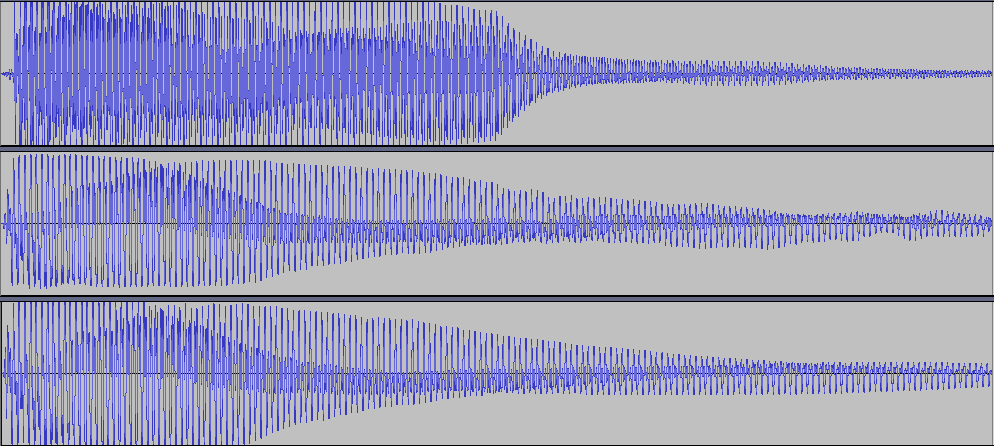
\includegraphics[width=0.9\hsize]{figure/88_88/f3.png}
\caption{F3の0.800秒から1.000秒までの音波}
\label{fig:88_88_good1}
\end{center}
\end{minipage}
\begin{minipage}{0.48\hsize}
\begin{center}
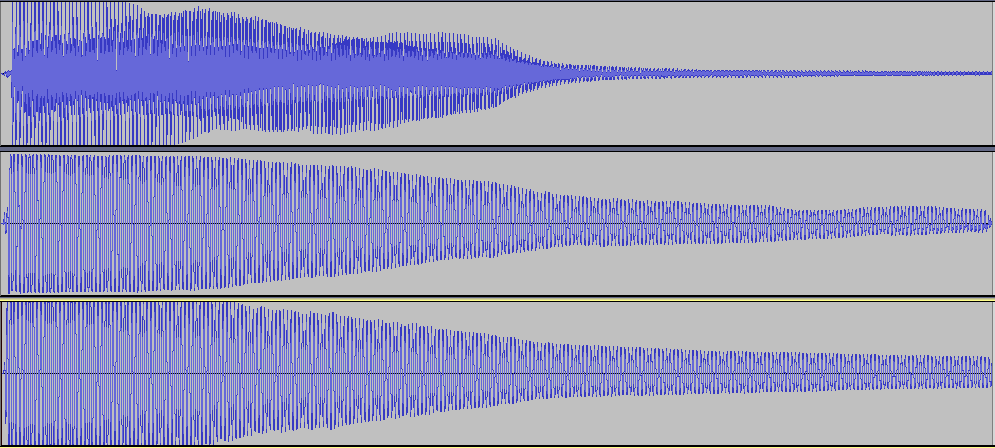
\includegraphics[width=0.9\hsize]{figure/88_88/c4.png}
\caption{C4の0.200秒から0.300秒までの音波}
\label{fig:88_88_good2}
\end{center}
\end{minipage}
\end{center}
\end{figure}


まず、F2からG6$\sharp$の音は耳で聴いても波形を見ても図\ref{fig:88_88_good1}のように正確にハープの音を表現することができていた。特にC4からD5$\sharp$の音は図\ref{fig:88_88_good2}のように上音の音が少ないために綺麗なハープの音を生成することができていた。他の音についても下記に挙げた改善点はあるものの基音の部分は表現することができていた。以下では、ハープの音を生成において困難であった点を列挙する。


\begin{description}

\item[音波の振幅]\mbox{}

\begin{figure}[t]
\begin{center}
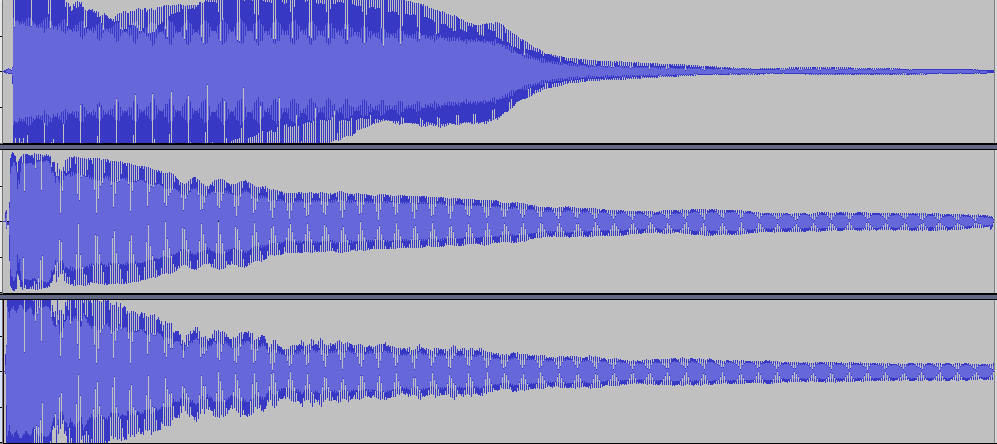
\includegraphics[width=0.7\hsize]{figure/88_88/c5.png}
\caption{C5の音波}
\label{fig:88_88_amp}
\end{center}
\end{figure}

図\ref{fig:88_88_amp}の波形の前半のように、生成された波形の振幅が小さいという問題が発生した。これにより、減衰していく部分の表現が難しい場合があった。原因は、振幅をランダムに小さくしたためであると考えられ、学習の初段階では振幅を固定するなどの工夫する必要があると思われる。
    
\item[音の鳴り出しの遅延]\mbox{}

\begin{figure}[t]
\begin{center}
\begin{minipage}{0.48\hsize}
\begin{center}
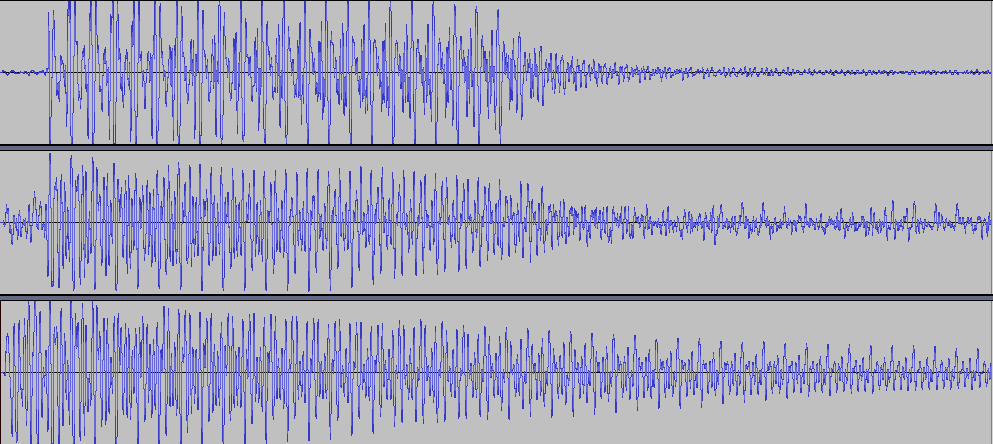
\includegraphics[width=0.9\hsize]{figure/88_88/f1s.png}
\caption{F1$\sharp$の0.000秒から1.000秒までの音波}
\label{fig:88_88_lag1}
\end{center}
\end{minipage}
\begin{minipage}{0.48\hsize}
\begin{center}
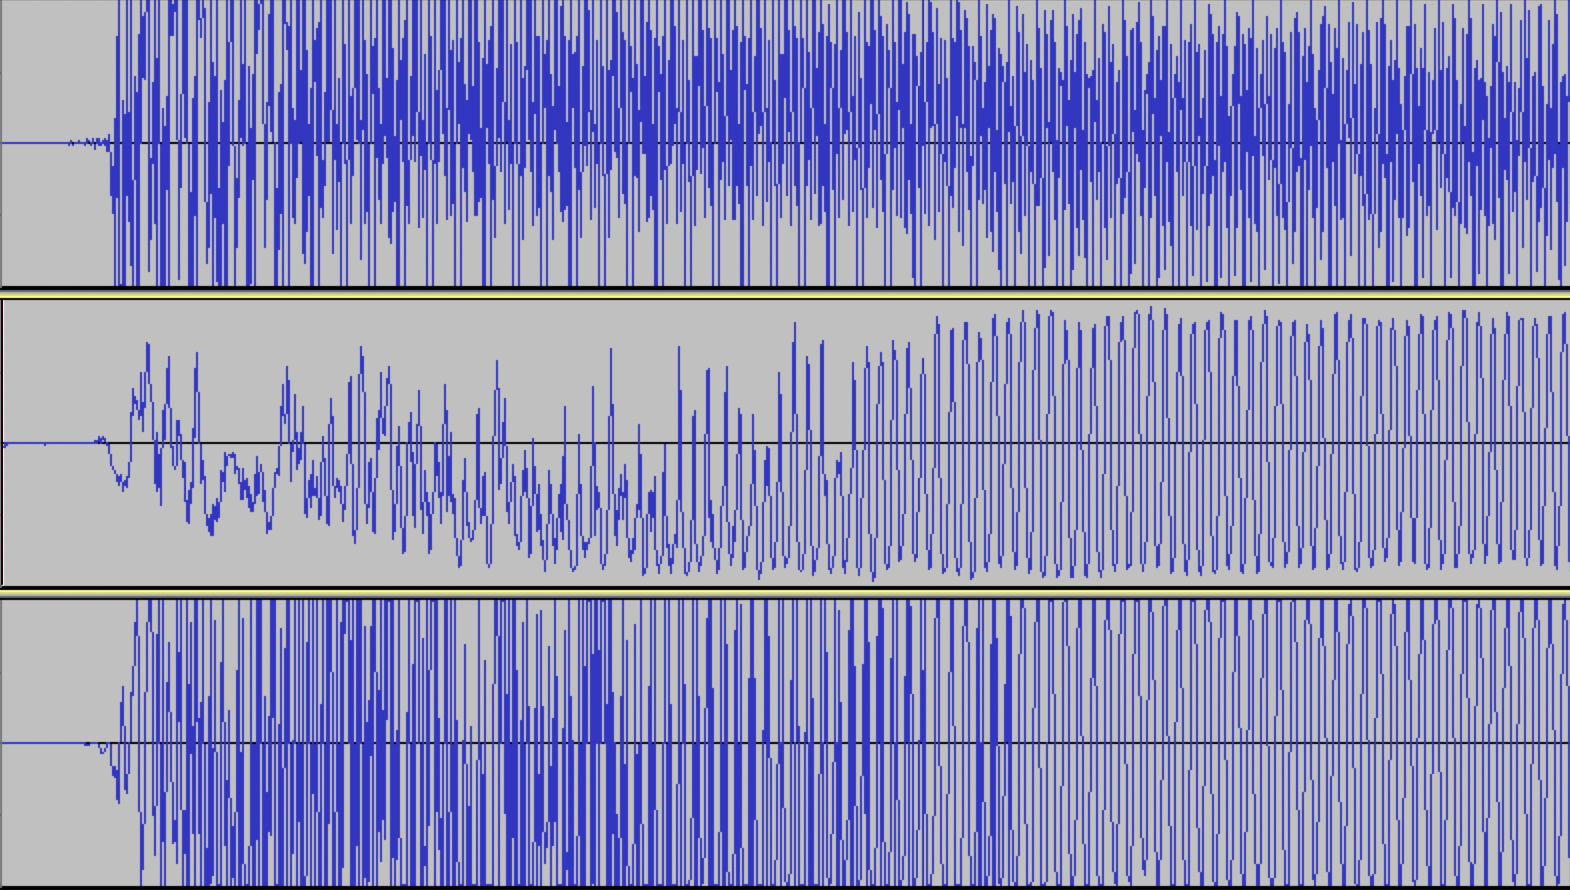
\includegraphics[width=0.9\hsize]{figure/88_88_det/a7_0_0030.png}
\caption{A7の0.000秒から0.030秒までの音波}
\label{fig:88_88_lag2}
\end{center}
\end{minipage}
\end{center}
\end{figure}

ギターとハープは弦楽器なので鳴り出すまでに遅延がある。特に、今回用いたデータセットでは図\ref{fig:88_88_lag1}のようにギターの音に遅延がある場合や図\ref{fig:88_88_lag2}のように周期的な音になるまでに遅延がある場合、その部分を学習することが難しかった。

\item[音波の滑らかさ]\mbox{}

\begin{figure}[t]
\begin{center}
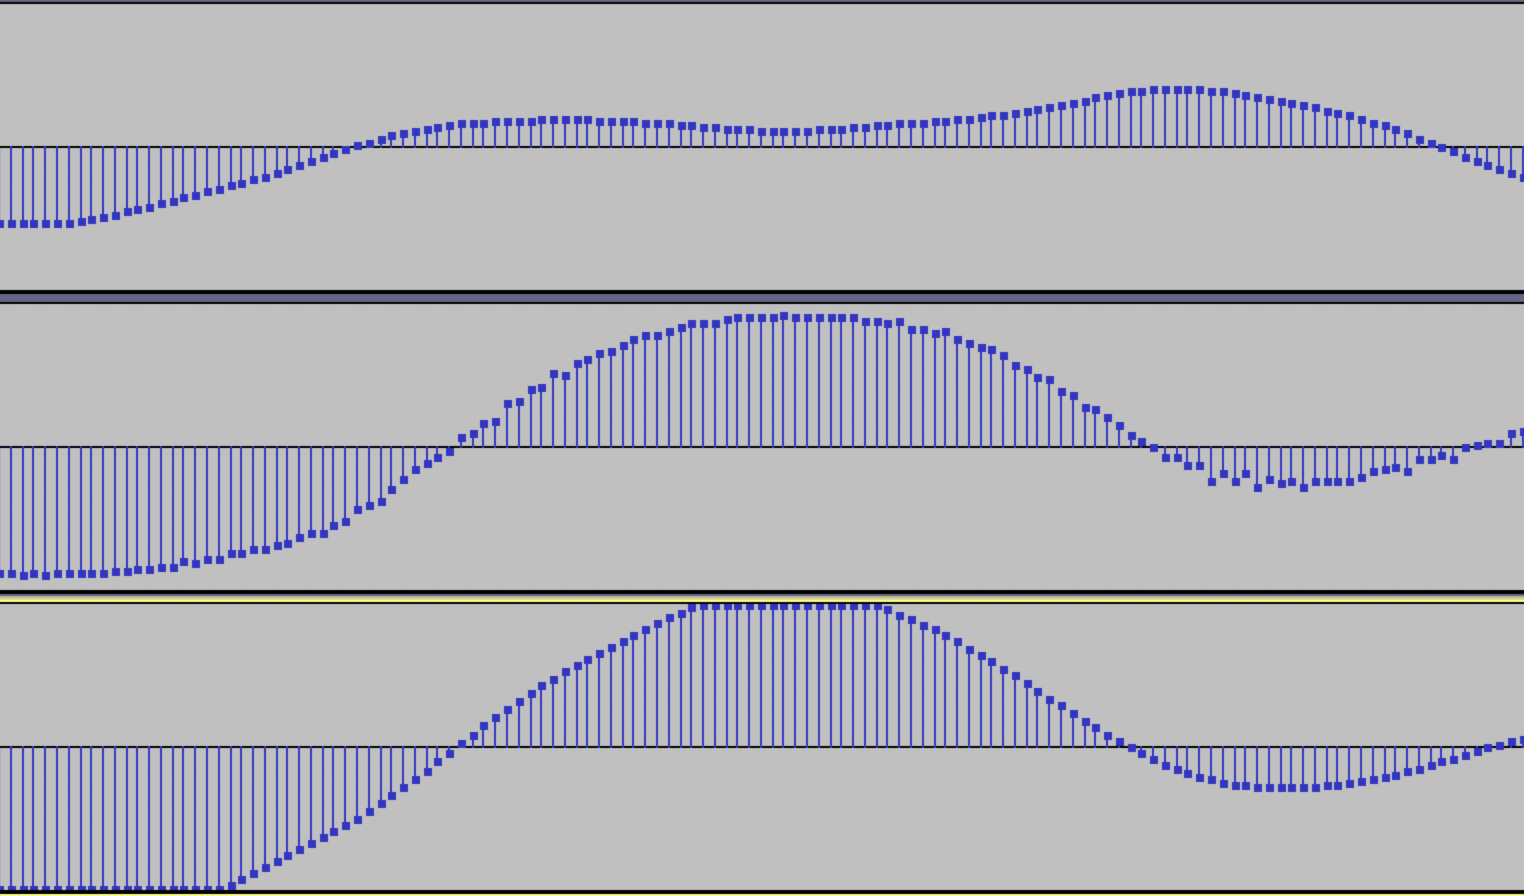
\includegraphics[width=0.7\hsize]{figure/88_88_det/d2s_0100_0103.png}
\caption{D2$\sharp$の0.100秒から0.103秒までの音波}
\label{fig:88_88_smooth}
\end{center}
\end{figure}

%滑らかさの表現
図\ref{fig:88_88_smooth}の上から2番目の波形と3番目の波形を比較すると、生成された波には滑らかさがないことがわかる。人間の耳にはこの滑らかでない音波の部分はノイズまじりの音として聞こえるので、この波を滑らかにするために工夫が必要であると考えられる。

\item[音波の振動の減衰]\mbox{}

\begin{figure}[t]
\begin{center}
\begin{minipage}{0.48\hsize}
\begin{center}
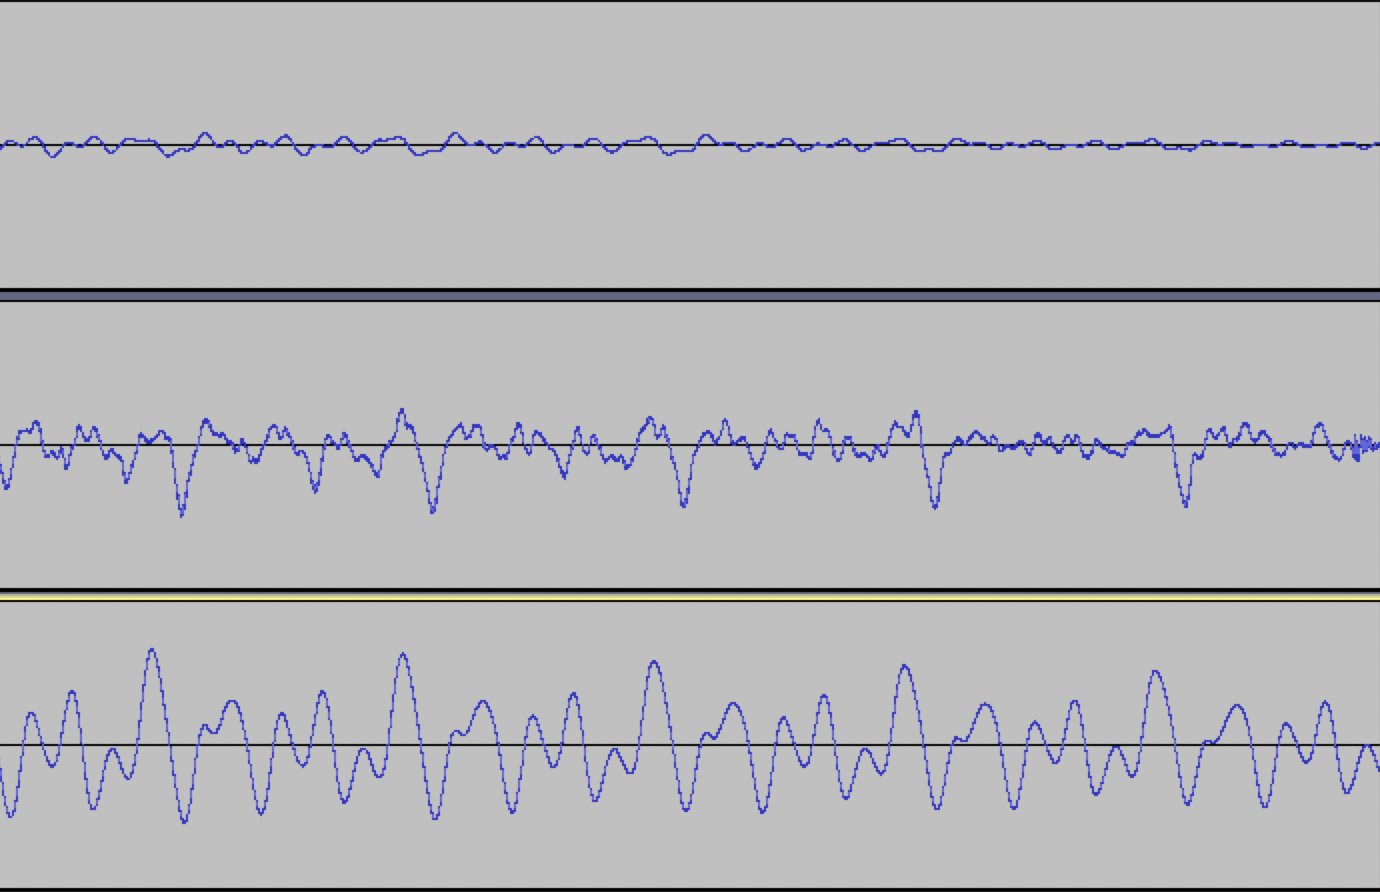
\includegraphics[width=0.9\hsize]{figure/88_88_det/a0_0800_1000.png}
\caption{A0の0.800秒から1.000秒までの音波}
\label{fig:88_88_reduce1}
\end{center}
\end{minipage}
\begin{minipage}{0.48\hsize}
\begin{center}
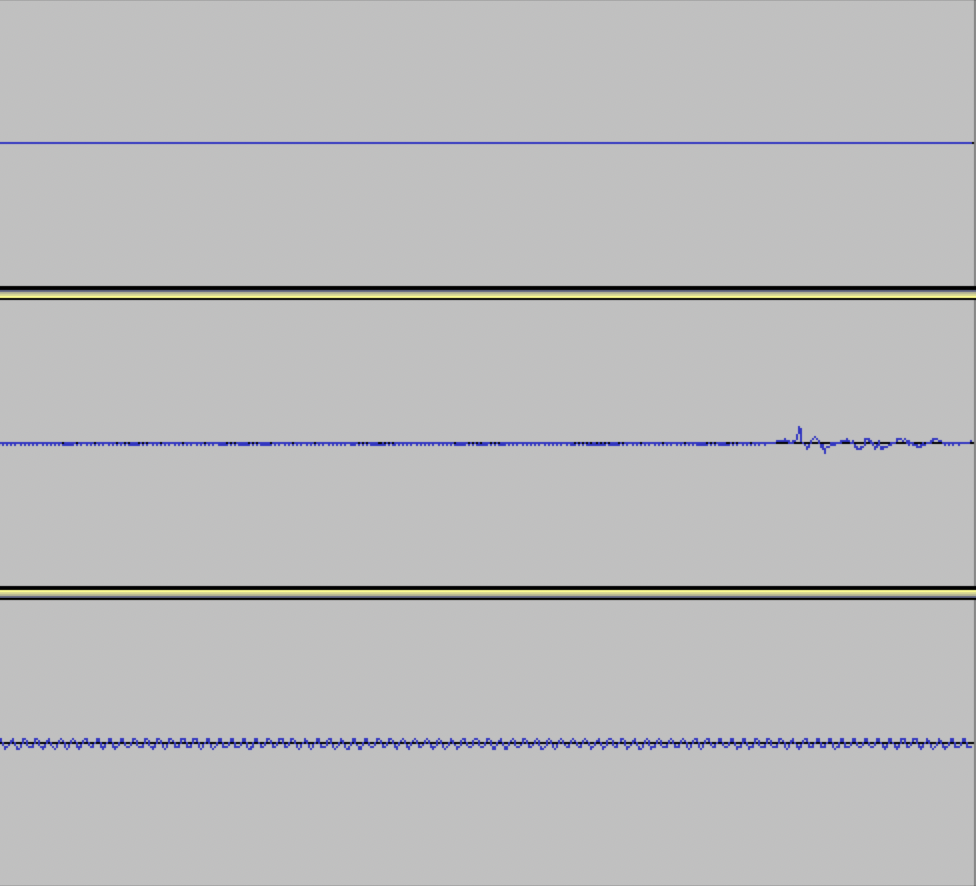
\includegraphics[width=0.9\hsize]{figure/88_88_det/b7_0980_1000.png}
\caption{B7の0.980秒から1.000秒までの音波}
\label{fig:88_88_reduce2}
\end{center}
\end{minipage}
\end{center}
\end{figure}

音波の振動の減衰が全く表現できていない音波があった。具体的には、A0,A0$\sharp$,B0,C1,C1$\sharp$,D1,D1$\sharp$,E1,\\
F1,F1$\sharp$,G1,G1$\sharp$D2,D2$\sharp$,E2,A6,A6$\sharp$,B6,C7,C7$\sharp$,D7,D7$\sharp$,F7,F7$\sharp$,G7,G7$\sharp$,A7,A7$\sharp$,B7,C8の音である。また、これ以外の音についても減衰が一部表現できていないものはあった。

これらの音のうち、E2以下の低音域の場合は図\ref{fig:88_88_reduce1}のようにハープとは全く異なる波形で減衰し、A6以上の高音域の場合は図\ref{fig:88_88_reduce2}のようにほとんど振動が見られなかった。原因としては、微小な振動をニューラルネットワークが学習するのが難しいことと今回のデータセットではギターの方がハープよりも音の鳴る時間が短かったことが挙げられる。

%ギターの方が全体的に短いならそれも表現されるはず
%高周波数の場合は変動が激しく学習が難しい
%初期のGANでは低解像度の画像しか作れなかったことに深く関連しそう
%高解像度の技術が適応可能?

\item[安定したデータセットの作成]\mbox{}

\begin{figure}[t]
\begin{center}
\begin{minipage}{0.48\hsize}
\begin{center}
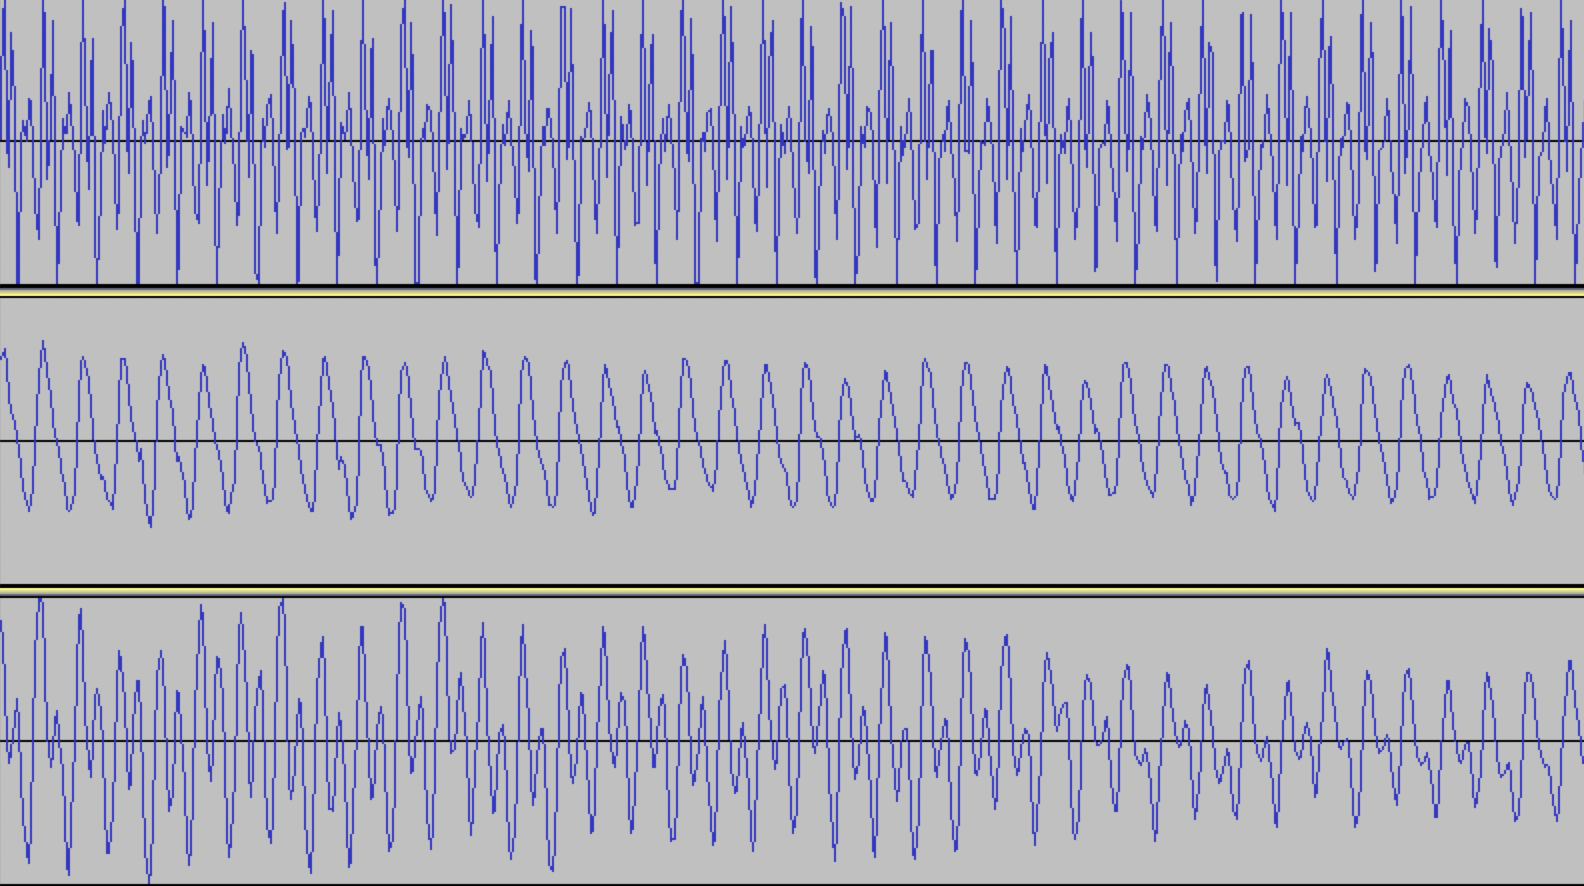
\includegraphics[width=0.9\hsize]{figure/88_88_det/e7_0550_0700.png}
\caption{E7の0.055秒から0.070秒までの音波}
\label{fig:88_88_bad1}
\end{center}
\end{minipage}
\begin{minipage}{0.48\hsize}
\begin{center}
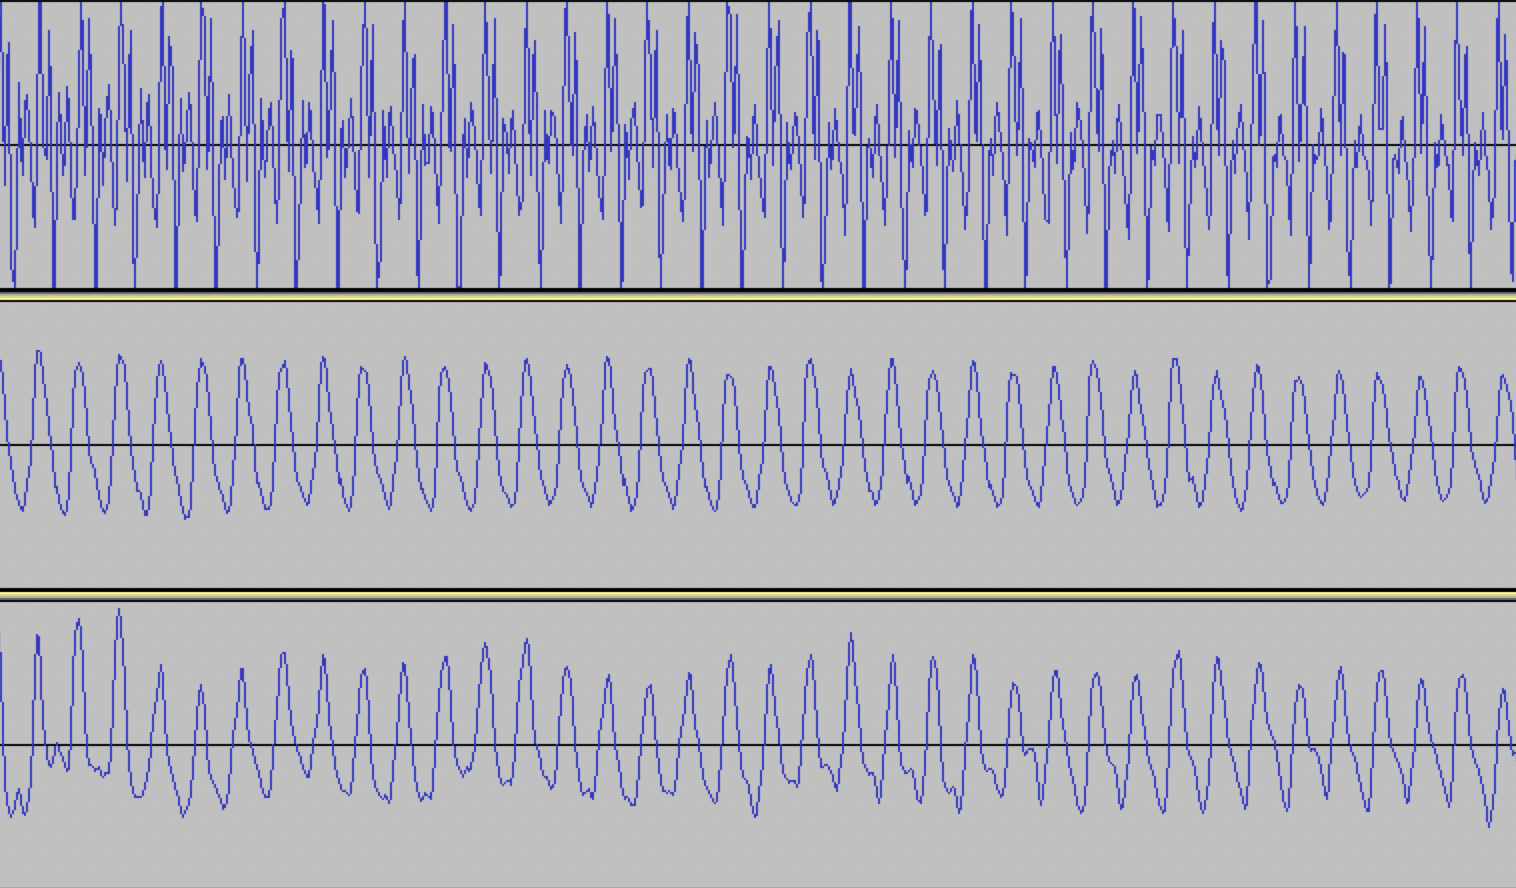
\includegraphics[width=0.9\hsize]{figure/88_88_det/d7s_0550_0700.png}
\caption{D7$\sharp$の0.055秒から0.070秒までの音波}
\label{fig:88_88_bad2}
\end{center}
\end{minipage}
\end{center}
\end{figure}

E7の音については、図\ref{fig:88_88_bad1}のように上記に挙げた以外の部分で波が表現できていなかったが、ハープのデータセットの音波の振動の振幅が安定していないために、ニューラルネットワークによる学習が難しかったと考えられる。

また、E7の半音下の音であるD7$\sharp$でも図\ref{fig:88_88_bad2}のようにハープのデータセットの音波の振動の振幅は安定しておらず、特に高音は安定した振幅のデータセットを生成することが難しいと考えられる。

\end{description}


\subsection{生成モデルの汎化能力}

まず、音の高さは変換前後で変わってないものが多く期待通りの結果となった。しかし、音の音色は元のギターの音色とは異なるもののハープに近い音色とは言い難い結果となり、\ref{sec:expression}節における課題も解決することはできなかった。以下では、生成されたハープの音についてそれぞれ考察を行う。

%学習の際のlossの図

\begin{description}
\item[音波の単純さ]\mbox{}

\begin{figure}[t]
\begin{center}
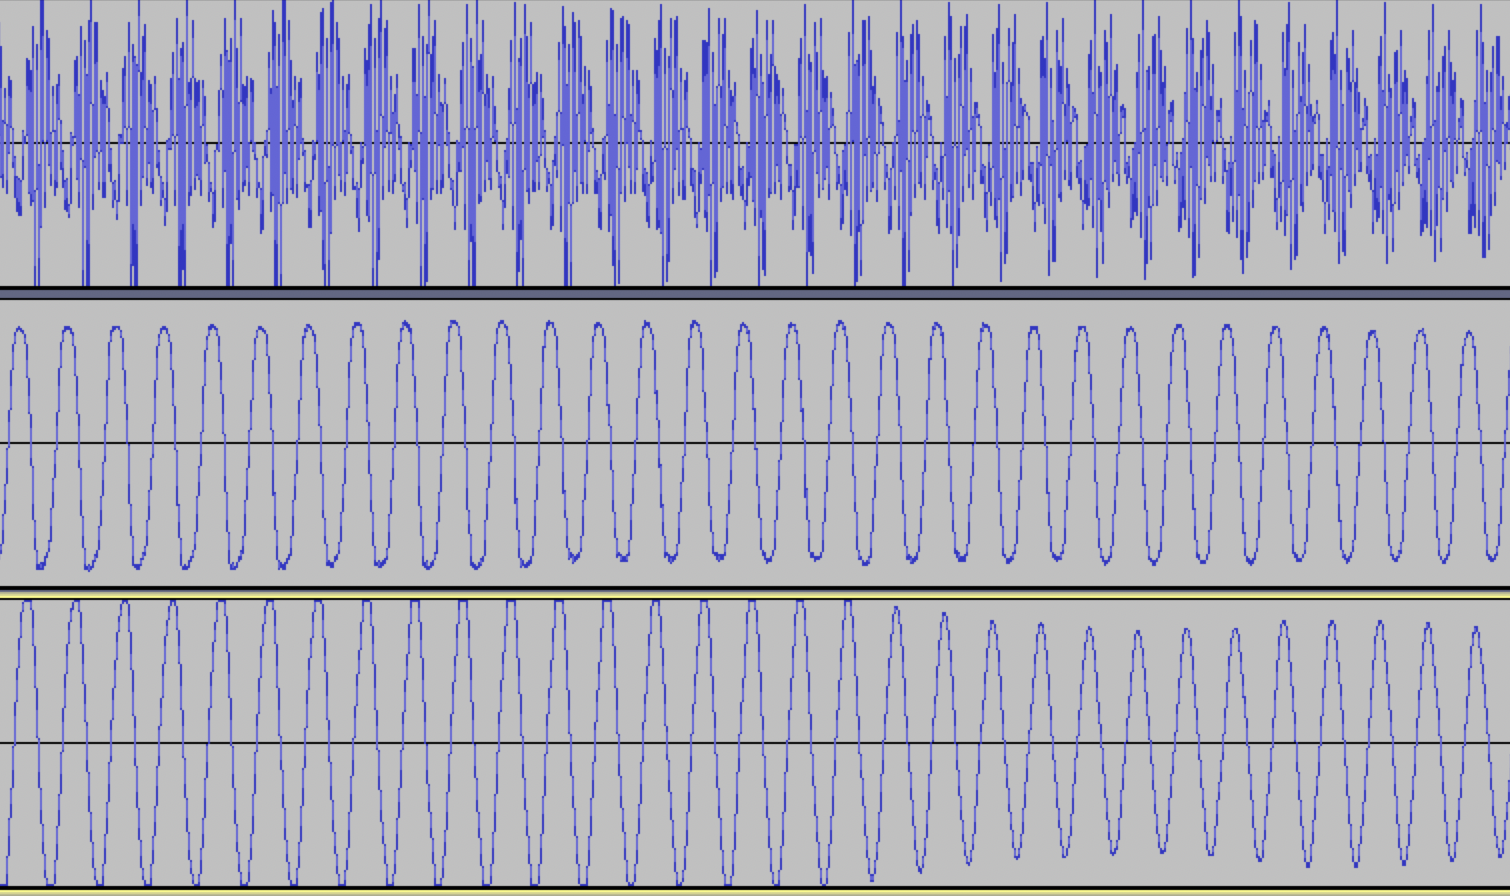
\includegraphics[width=0.7\hsize]{figure/66_22_det/d4s_0100_0200.png}
\caption{D4$\sharp$の0.100秒から0.200秒までの音波}
\label{fig:66_22_near}
\end{center}
\end{figure}

\ref{sec:expression}節と同程度にハープに近い音が生成される場合もあった。具体的には、D4,D4$\sharp$,G4,F5,F5$\sharp$の音である。これらの音は音波が図\ref{fig:66_22_near}のように単純な波形でニューラルネットワークによる表現が容易であるため、生成が他の音波に比べて容易であったと考えられる。

\item[音波の複雑さ]\mbox{}

\begin{figure}[t]
\begin{center}
\begin{minipage}{0.48\hsize}
\begin{center}
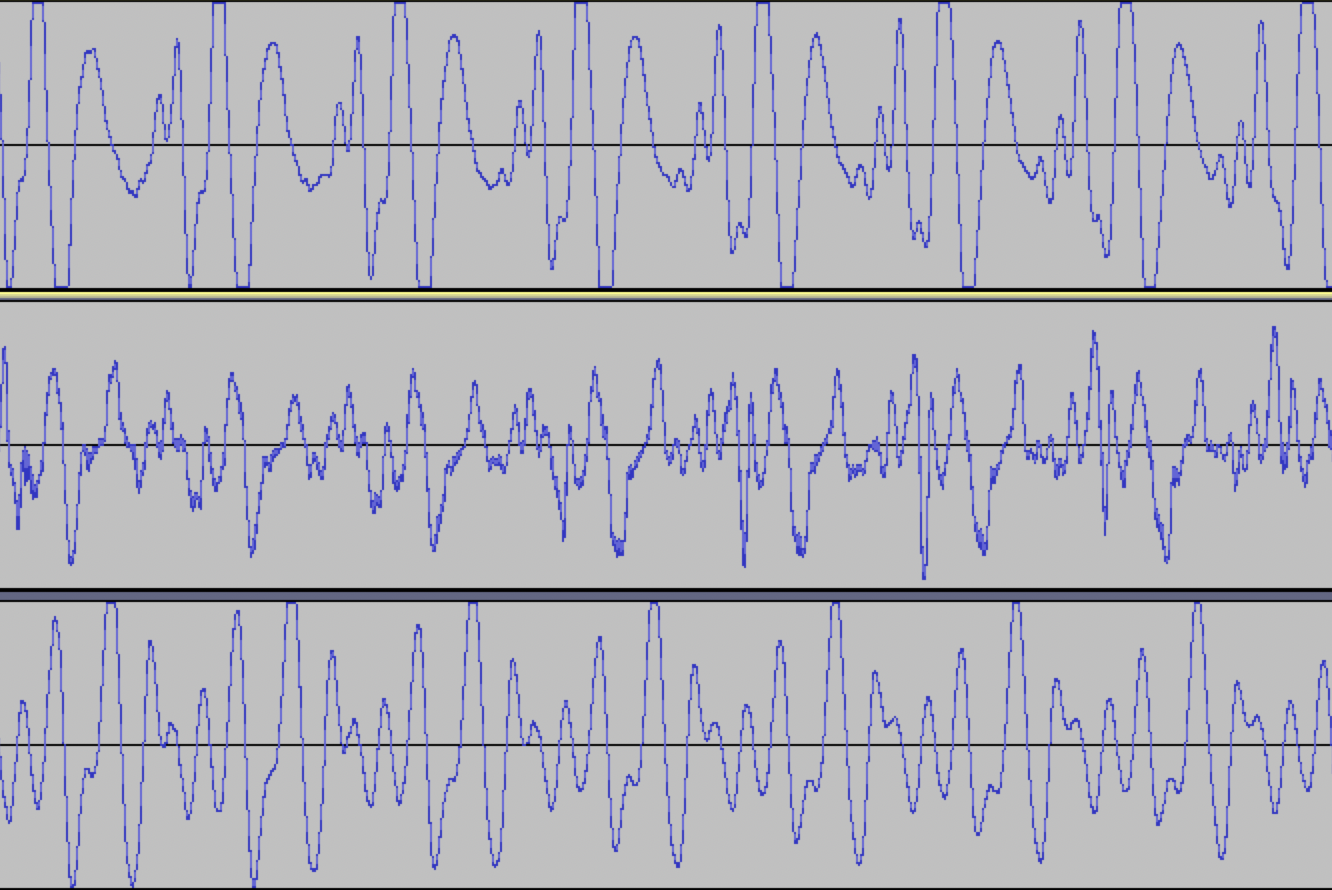
\includegraphics[width=0.9\hsize]{figure/66_22_det/d1_0300_0500.png}
\caption{D1の0.300秒から0.500秒までの音波}
\label{fig:66_22_bad1}
\end{center}
\end{minipage}
\begin{minipage}{0.48\hsize}
\begin{center}
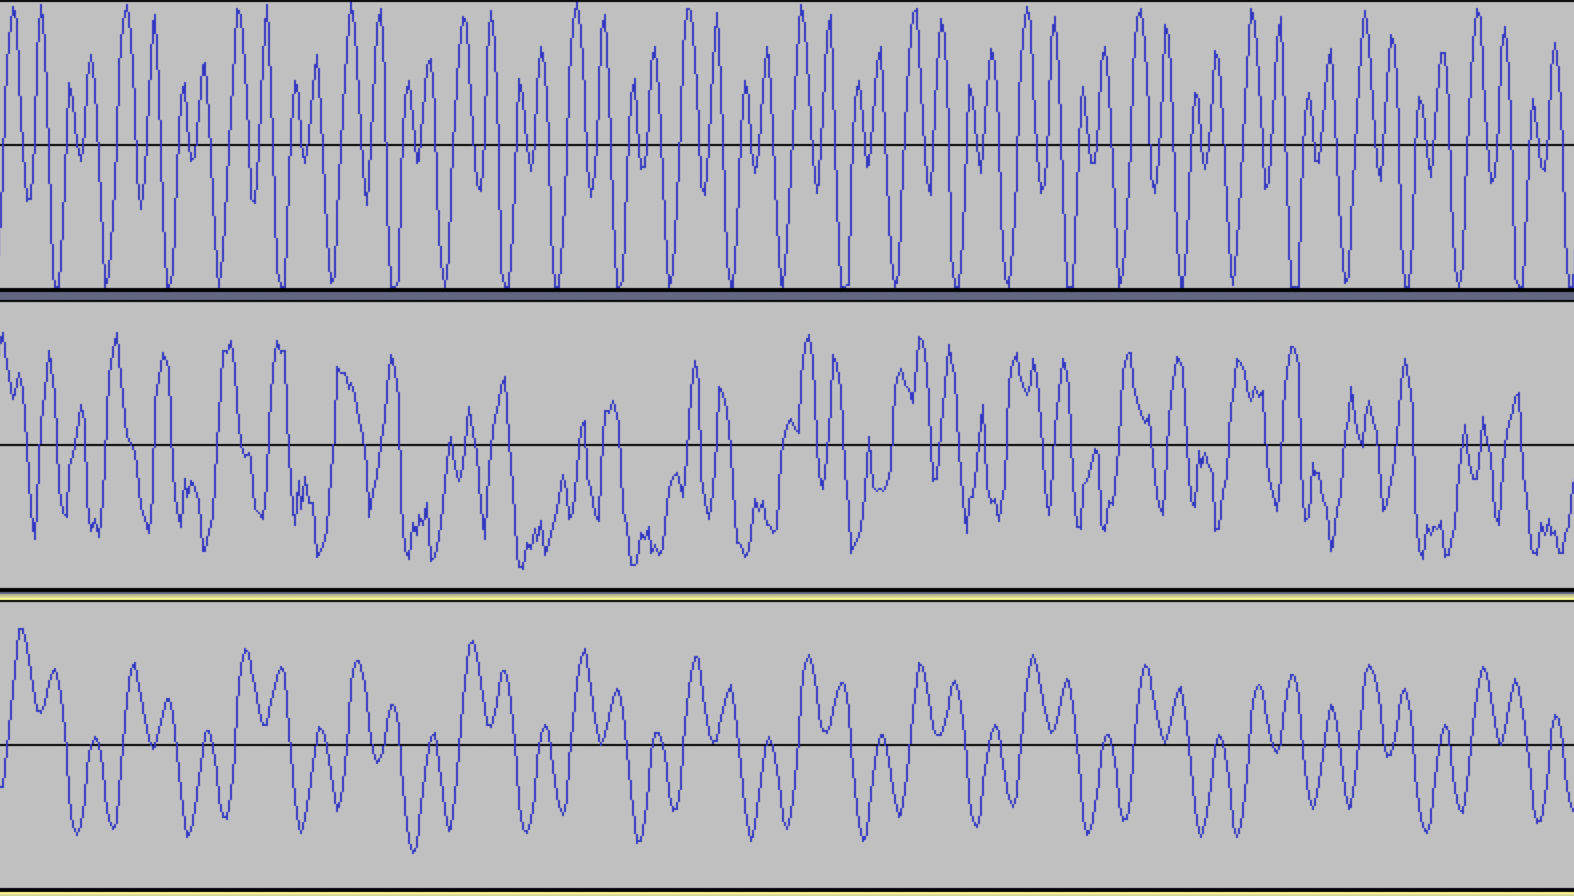
\includegraphics[width=0.9\hsize]{figure/66_22_det/f6_0070_0080.png}
\caption{F6の0.070秒から0.080秒までの音波}
\label{fig:66_22_bad2}
\end{center}
\end{minipage}
\end{center}
\end{figure}

\begin{figure}[t]
\begin{center}
\begin{minipage}{0.48\hsize}
\begin{center}
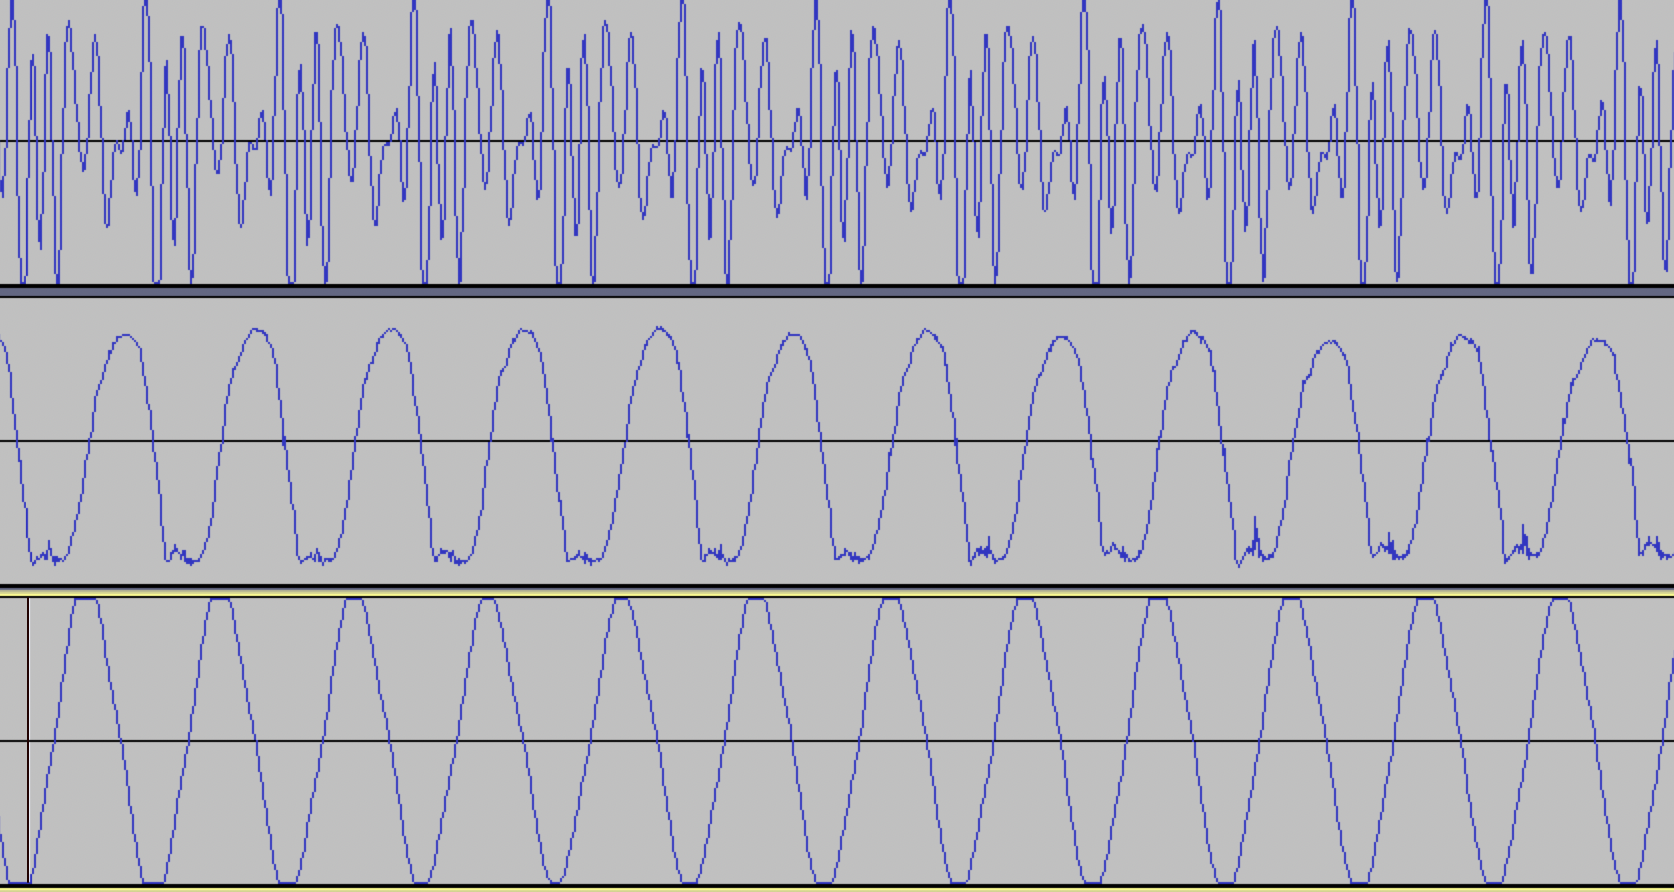
\includegraphics[width=0.9\hsize]{figure/66_22_det/g4s_0150_0180.png}
\caption{G4$\sharp$の0.150秒から0.180秒までの音波}
\label{fig:66_22_bad3}
\end{center}
\end{minipage}
\begin{minipage}{0.48\hsize}
\begin{center}
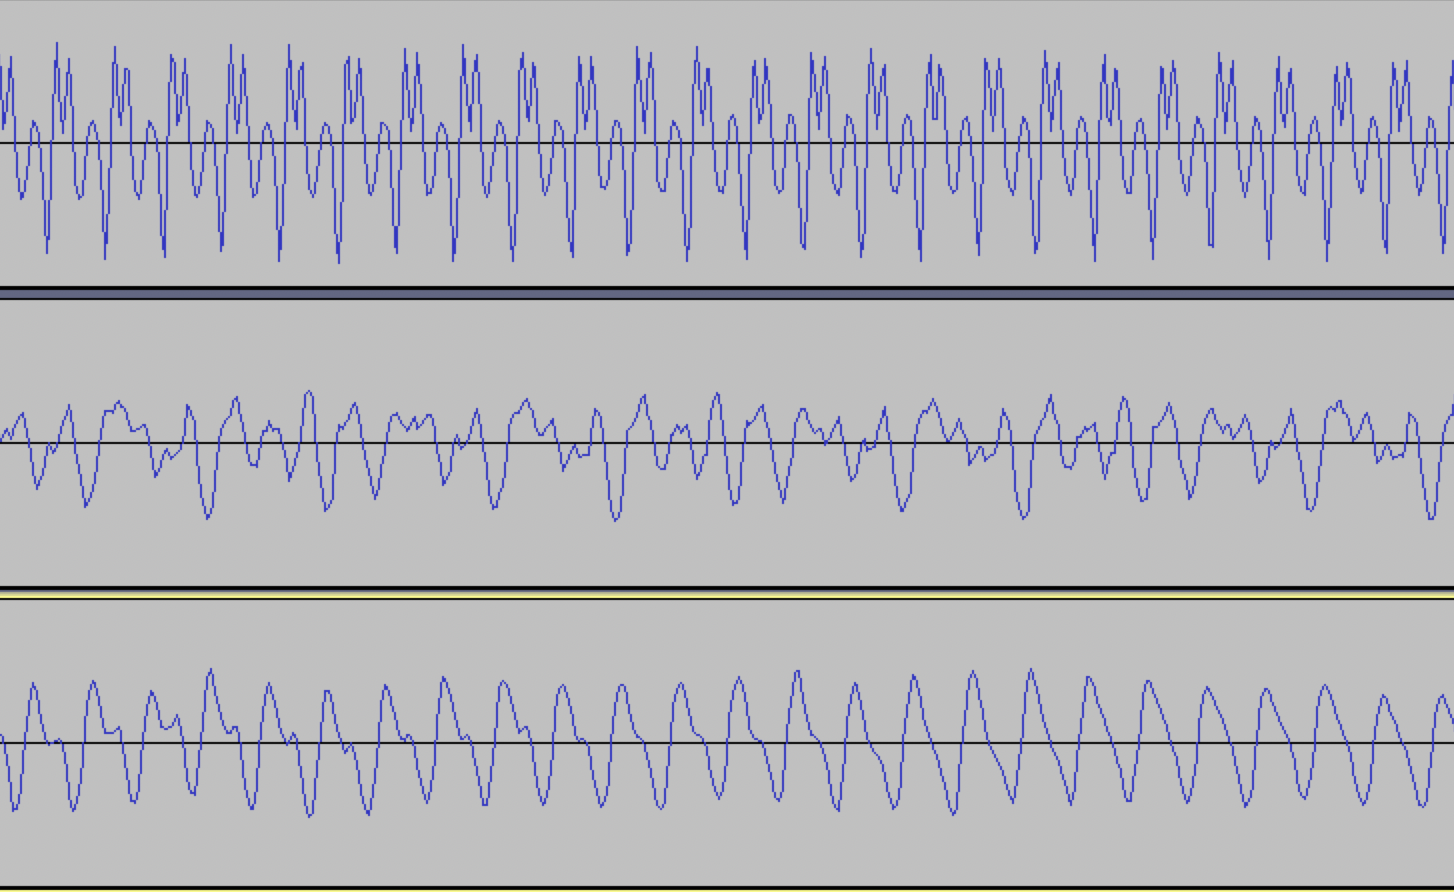
\includegraphics[width=0.9\hsize]{figure/66_22_det/d7s_0100_0110.png}
\caption{D7$\sharp$の0.1700秒から0.110秒までの音波}
\label{fig:66_22_bad4}
\end{center}
\end{minipage}
\end{center}
\end{figure}

上記の単純な音波以外の場合はハープとは言い難い音が生成された。いくつか種類があったが、図\ref{fig:66_22_bad1}や図\ref{fig:66_22_bad2}のように、音波が安定した振動をせず上音の成分がハープよりも多い音波が多く観測された。

また、ほとんどの音波において基音の位相は保たれていたが、図\ref{fig:66_22_bad3}のように位相が異なる音波や図\ref{fig:66_22_bad4}のように基音が異なる音波が生成されることもあった。

これらの原因は、振幅をランダムにすることにより学習が安定しないことと微細な表現を可能なニューラルネットワークを構築できていないためと考えられる。

\end{description}